\documentclass{beamer}
\usepackage[utf8]{inputenc}
\usepackage{amsmath}
\usepackage{amsfonts}
\usepackage{amssymb}
\usepackage{amsthm}
\usepackage[russian]{babel}
\usepackage{hyperref}
\usepackage{enumerate}
\usepackage{graphicx}
\usepackage{float}
\usepackage{wrapfig}
\usepackage{natbib}
\usepackage{bibentry}
\usepackage{url}
\usetheme{Madrid}

\begin{document}
\title{Каталоги шаровых скоплений}
\author[Фархутдинова, Кочергина, Дромашко]{Фархутдинова~А.~М. \and Кочергина~П.~B. \and Дромашко~M.~C.}
\institute{Санкт-Петербургский государственный университет}
\date{29 февраля 2024}
\maketitle
\begin{frame}
    \frametitle{Содержание}
    \tableofcontents
\end{frame}
    \section{История}
    \begin{frame}{История}
        \begin{columns}
            % Column 1
            \begin{column}{0.6\textwidth}
                    \begin{enumerate}[]
                        \item Первым открытым считается M22 (изначально принято за туманность) \par Johann Abraham Ihle, 1665
                        \item Омега Центавра (NGC 5139) \par Edmond Halley, 1677
                        \item M5 в Голове Змеи \par Gottfried Kirch, 1702
                        \item M13 в Геркулесе \par Edmond Halley, 1714
                    \end{enumerate}
            \end{column}
            % Column 2    
            \begin{column}{0.4\textwidth}
                \begin{figure}
                \centering
                    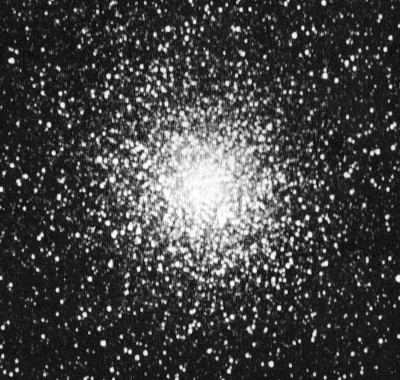
\includegraphics[width=0.6\textwidth]{pictures/m22.jpg}
                    \caption{Шаровое скопление M22}
                \end{figure}
            \end{column}
        \end{columns}
    \end{frame}
    \begin{frame}{История}
                    \begin{enumerate}[]
                        \item Список ``Тумманостей'' (21 обьект)\cite{list21}. Два новых шаровых скопления M71 и M4 \par De Chéseaux, 1746
                        \item M15 и M2 \par Jean-Dominique Maraldi, 1746 
                        \item Каталог южных ``туманностей''. 7 шаровых скоплений (среди них 4 новых). \par Nicholas Louis de Lacaille, 1751-52
                        \item Каталог Тумманостей и Звездных Скоплений (110 обьектов). 29 шаровых скоплений из которых 20 --- новые открытия. \par Charles Messier, 1774
                    \end{enumerate}
                    Шарль Мессье первым разрешил шаровое скопление M4, но все же называл остальные 28 таких объектов в своем каталоге ``круглыми туманностями''.
    \end{frame}
    \begin{frame}{История}
        \begin{figure}
            \centering
                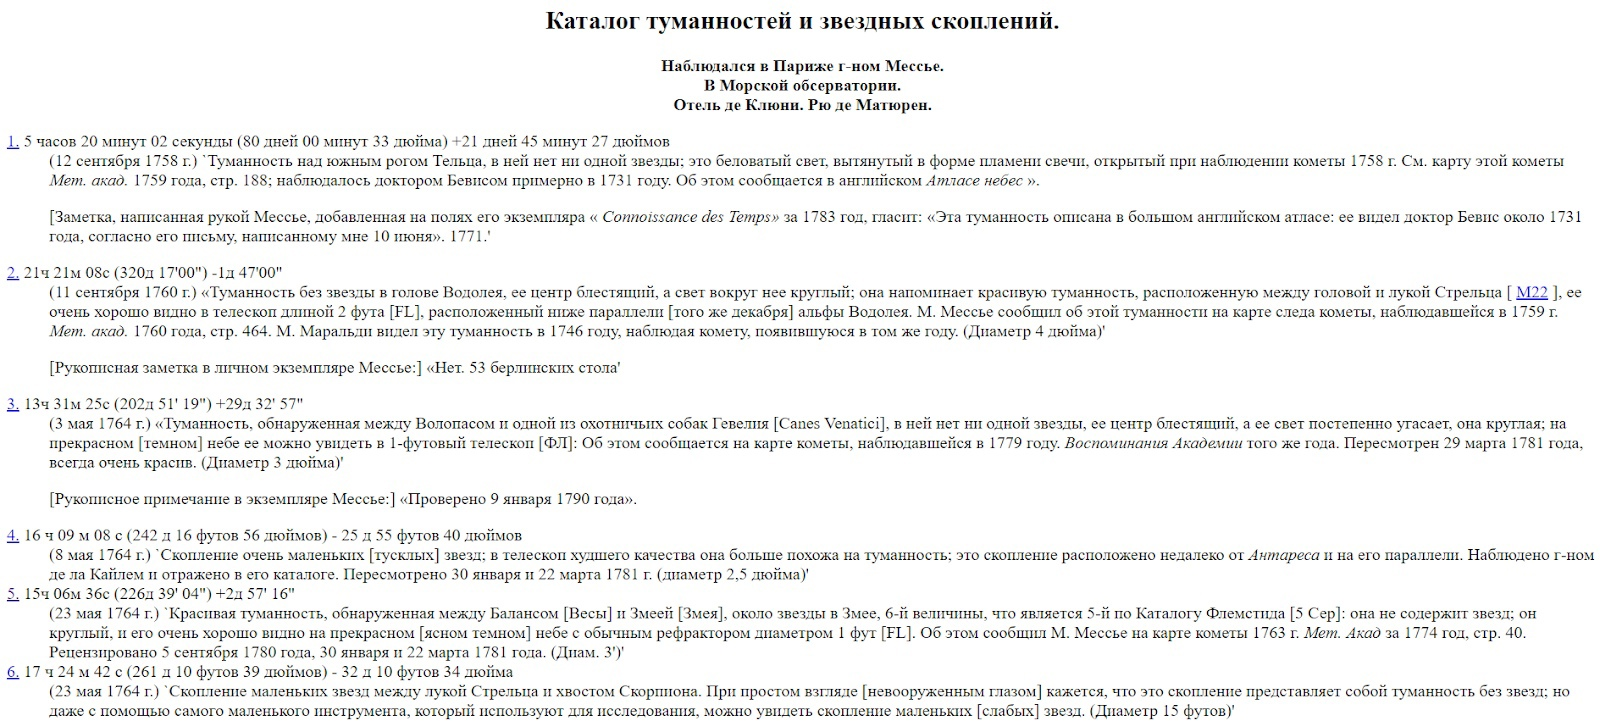
\includegraphics[width=0.9\linewidth]{pictures/Messie.jpg}
            \end{figure}
    \end{frame}
    \begin{frame}{История}
        \begin{columns}
                % Column 1
            \begin{column}{0.7\textwidth}
                Таким образом, летом 1782 года, до того как Уильям Гершель начал свое всестороннее исследование неба, 
                было известно 34 шаровых скопления. Сам Гершель открыл 36 новых шаровиков. Он был первым, кто разрешил практически все из них в звезды, 
                и ввел термин «шаровое скопление» в дискуссии, 
                связанной с его вторым каталогом из 1000 объектов глубокого космоса (1789).
            \end{column}
                % Column 2    
            \begin{column}{0.3\textwidth}
                \begin{figure}
                    \centering
                    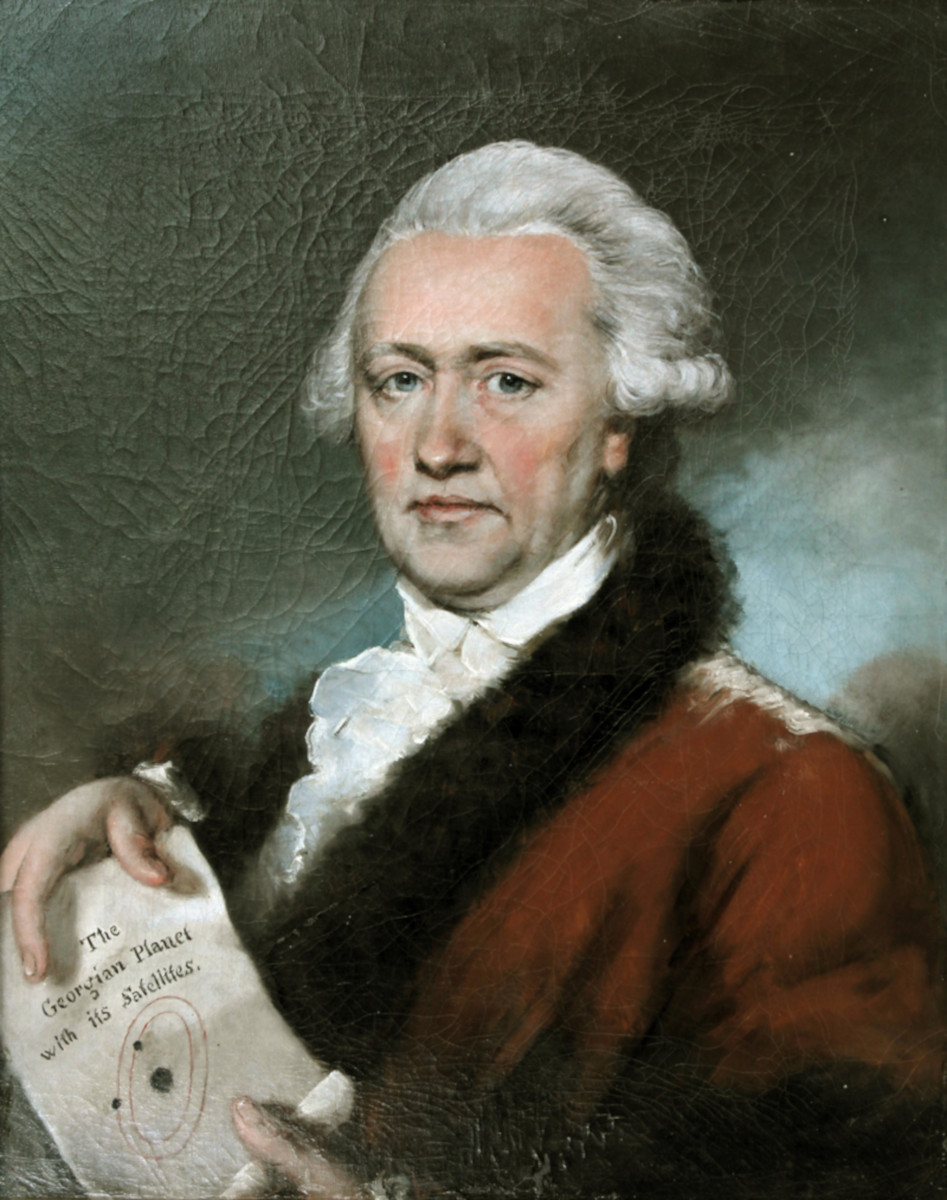
\includegraphics[width=0.7\textwidth]{pictures/Gersh.jpg}
                \end{figure}
            \end{column}
        \end{columns}
    \end{frame}
    \begin{frame}{История}
        Все эти ранние известные шаровые звезды принадлежат нашей Галактике, 
        но некоторые из них были интегрированы или иммигрировали в систему галактического шарового скопления лишь недавно, 
        включая M54 (отмечено в 1994 году) и M79 (отмечено в 2003 году).
    \end{frame}
    \begin{frame}{История}
        \begin{enumerate}[]
            \item Каталог Меллота (1915)\cite{Mellot1915} содержит около 82 шаровых скоплений.
            \item Каталог Шепли (1930)\cite{Shapley1930} --- 93 скопления.
            \item Хелен Сойер\cite{Hogg1947} перечисляет 99 шаровых скоплений Млечного Пути, 97 из которых до сих пор считаются таковыми; в ее списке 1959 года\cite{Hogg1959} 118 записей (115 реальных).
            \item Дальнейшие списки Арпа (1965) , Алькаино (1973) и Кукаркина (1974) содержат от 119 до 131 кластера.
            \item Беквар перечисляет 100 шаровых скоплений.
            \item Каталог неба 2000.0 перечисляет 138 шаровых объектов, число, указанное для 1987 года также Кеннетом Глином Джонсом (1991)
        \end{enumerate}
    \end{frame}
    \begin{frame}{История}
        \begin{enumerate}[]
            \item База данных У.Э. Харриса за 1994 год содержит 142 объекта (те же 141 реальный объект), за 1996 и 1997 годы — 146, за версию 1999 года — 147, за февраль 2003 г. — 150, а за самую последнюю версию (декабрь 2010 г.) — 157, причем еще 8 кандидатов еще недостаточно подтверждены
            \item Текущий каталог Хольгера Баумгардта содержит данные для 168 шаровых скоплений Галактики \cite{Baumgardt2023}
        \end{enumerate}
        Из 168 известных шаровых скоплений Галактики 104 находятся в каталоге NGC, а еще 3 — в каталоге IC JLE Dreyer.
    \end{frame}
    \section{Малые каталоги}
    \begin{frame}{Малые каталоги. Palomar globular clusters}
        \begin{enumerate}[]
            \item Одни из самых слабых шаровых скоплений в Галактике.
            \item Были обнаружены в 1950-х годах на обзорных пластинках первого обзора неба Паломарской обсерватории (POSS).
            \item Всего 15 шаровых скоплений.
            \item Некоторые произошли из другой галактики, например, Паломар~12 из карликовой сфероидальной галактики Стрельца.
        \end{enumerate}
    \end{frame}
    \begin{frame}{Малые каталоги. Palomar globular clusters}
        \begin{figure}[h]
            \centering
            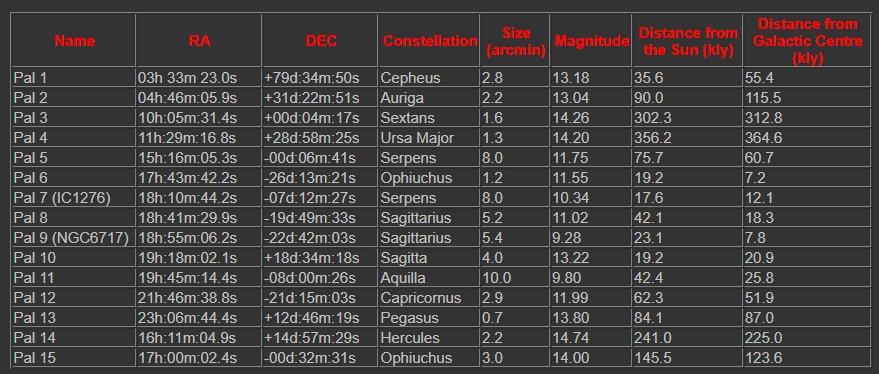
\includegraphics[width=0.9\linewidth]{pictures/PGC.jpg}
        \end{figure}
    \end{frame}
    \begin{frame}{Малые каталоги. 2MASS-GC и HVGC}
        \begin{enumerate}[]
            \item 2MASS-GC --- два шаровых скопления 2MASS-GC01 и 2MASS-GC02, найденных из обзора неба 2MASS в ИК. Находятся в плоскости галактического диска.
            \item HVGC (Hyper velocity globular clusters) --- на данный момент только одно скопление в галактике Messier 87 в созвездии Девы. 
        \end{enumerate}
    \end{frame}
    \begin{frame}{Малые каталоги. Arp 1965}
        \begin{enumerate}[]
            \item Опубликован Халтоном К. Арпом в 1965 году как часть обзорной статьи по шаровым скоплениям.
            \item Представляет собой усовершенствованную версию предыдущей публикации г-жи Хогг (1959)\cite{Hogg1959}
            \item Оценка полноты каталога составляет $98$\% для галактических широт выше $b(II) = 8$ градусов и $94$\% для низких широт для классов концентрации ниже XI.
            \item В обзоре основное внимание уделялось чуть более чем сотне примерно сферических звездных скоплений, интегральный показатель цвета которых находится в диапазоне B-V $0,6 - 0,8$ магнитной величины, а собственная звездная величина - от -4 до -10 магнитных величин.
        \end{enumerate}
    \end{frame}
    \begin{frame}{Малые каталоги. Terzan}
        \begin{enumerate}[]
            \item 11 шаровиков, открытых Агопом Терзаном (Франция) в инфракрасном диапазоне.
            \item Cкопления сильно скрыты и расположены близко к Галактическому центру. 
            \item Первоначально было 12 записей, из которых оригинальный Терзан 11 был повторным открытием Терзана 5; в новых списках первоначальный Терзан 12 перенумерован на Терзан 11.
            \item Наблюдения проводились в ближнем ИК на 193 сантиметровом телескопе Обсерватории Верхнего Прованса и 48 дюймовым телескопе шмидта в Маунт-Паломар. 
        \end{enumerate}
    \end{frame}
    \begin{frame}{Малые каталоги. Terzan}
        \begin{figure}[h]
            \centering
            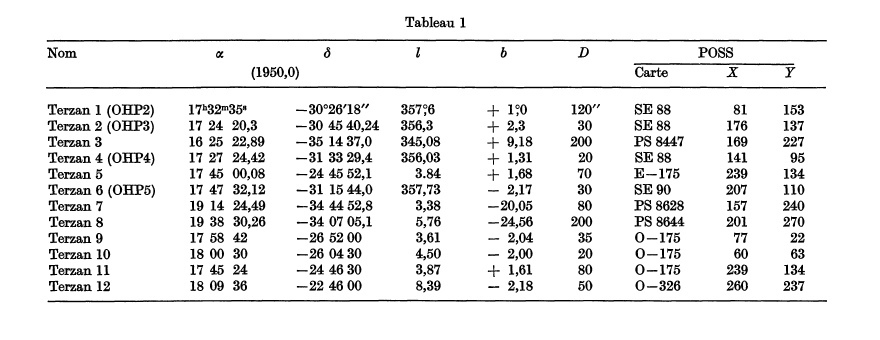
\includegraphics[width=0.9\linewidth]{pictures/Terzan.jpg}
        \end{figure}
    \end{frame}
    \begin{frame}{Малые каталоги. Djorg}
        \begin{enumerate}[]
            \item Наблюдались в полосах V, R, I на 1.5 метровом телескопе.
            \item Экспозиции от 1 минуты до 10 минут.
        \end{enumerate}
        \begin{figure}[h]
            \centering
            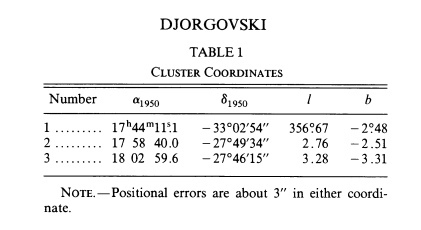
\includegraphics[width=0.7\linewidth]{pictures/Djorg.jpg}
        \end{figure}
    \end{frame}
    \section{Каталог Harris}
    \section{Список литературы}
    \begin{frame}[t, allowframebreaks]{Список литературы}
        \bibliographystyle{plain}
        \bibliography{bibliography}
    \end{frame}
\end{document}